% video/slides.tex -- slides for the team video (<= 5 minutes). Spoken text: video/SCRIPT.md.
% Build: video/RECORDING.md, section 2 (XeLaTeX in an ASCII folder; the project path is not ASCII).
%
% Page = PowerPoint widescreen (13.333 x 7.5 in), so point sizes mean what they mean in PowerPoint:
% body text 20-26 pt, slide titles 30 pt, source lines 13 pt.
% The bottom-right corner (3.0 x 1.7 in, about 430 x 245 px in a 1080p recording) is kept empty on every
% slide for the speaker's camera; set \camguidetrue below to see it while rehearsing.
% Figures: reports/figures/*.png, written by the scripts and runs named in each slide's source line.
% Numbers: each one traces to the run, submission or table in the source line and in video/SCRIPT.md, "Sources".
% Drafted 2026-11-01 by Claude Code (Anthropic, Claude Opus 5.5), workflow agent video_kit. Members edit the
% block below, rebuild, and must be able to explain every slide (Kaggle rule 6).

\documentclass[20pt,t]{beamer}
\geometry{paperwidth=13.333in,paperheight=7.5in}

%======================= EDIT HERE (team) =======================
\newcommand{\TeamName}{TODO\_TEAM\_NAME}
\newcommand{\KaggleTeam}{TODO\_KAGGLE\_TEAM\_NAME}
\newcommand{\NameA}{TODO\_NAME\_A}   % speaker A (full name as in the report)
\newcommand{\NameB}{TODO\_NAME\_B}   % speaker B; 1-member team: leave empty {}
\newcommand{\NameC}{TODO\_NAME\_C}   % speaker C; 1- or 2-member team: leave empty {}
\newcommand{\OwnerEone}{TODO owner}  % member who owns E1 (only owned extensions are shown)
\newcommand{\OwnerEtwo}{TODO owner}
\newcommand{\OwnerEthree}{TODO owner}
\newcommand{\OwnerEfour}{TODO owner}
% true = slide shown. Set an extension to false when no member owns it (1-3 members own 1-3 extensions).
\newif\ifEone   \Eonetrue
\newif\ifEtwo   \Etwotrue
\newif\ifEthree \Ethreetrue
\newif\ifEfour  \Efourtrue
% Last slide: one sentence per member, as that member will say it (empty {} = line not shown).
\newcommand{\TakeA}{A 0.01 difference needs repeated, paired cross-validation.}
\newcommand{\TakeB}{395 public rows catch bugs; they cannot rank good models.}
\newcommand{\TakeC}{Here, unlabelled rows were worth more than labels.}
\newif\ifcamguide \camguidefalse      % true = outline the camera corner (rehearsal only)
%================================================================

\usepackage{lmodern}               % scalable fallback fonts (avoids size-substitution warnings)
\usepackage{fontspec}
\setsansfont{Calibri}
\setmainfont{Calibri}
\usefonttheme{professionalfonts}
\usepackage{booktabs,array,etoolbox}
\usepackage{tikz}
\usetikzlibrary{positioning,arrows.meta,calc,decorations.pathreplacing}
\graphicspath{{../reports/figures/}{figures/}}

\definecolor{ink}{HTML}{1F2328}
\definecolor{muted}{HTML}{59636E}
\definecolor{accent}{HTML}{1F6FD1}
\definecolor{accent2}{HTML}{D9581F}
\definecolor{soft}{HTML}{EAF1FB}

\title{Small-Sample Classification Challenge: video slides}   % PDF metadata only (slide 1 is drawn by hand)
\author{Team \TeamName}
\hypersetup{pdfsubject={DSAI4203 team video; drafted with Claude Code (AI), see the report's AI disclosure}}

\setbeamertemplate{navigation symbols}{}
\setbeamersize{text margin left=0.55in,text margin right=0.55in}
\setbeamercolor{normal text}{fg=ink,bg=white}
\setbeamercolor{structure}{fg=accent}
\setbeamercolor{frametitle}{fg=ink}
\setbeamerfont{frametitle}{size=\fontsize{30}{35}\selectfont,series=\bfseries}
\setbeamerfont{framesubtitle}{size=\fontsize{20}{24}\selectfont,series=\mdseries}
\setbeamertemplate{itemize item}{\raisebox{0.12em}{\color{accent}\rule{0.42em}{0.42em}}}
\setlength{\leftmargini}{1.05em}
% no hyphenation on slides; allow looser lines instead
\hyphenpenalty=10000 \exhyphenpenalty=10000 \tolerance=9000 \emergencystretch=2em

\makeatletter
\setbeamertemplate{frametitle}{%
  \vspace*{0.30in}%
  {\usebeamerfont{frametitle}\usebeamercolor[fg]{frametitle}\insertframetitle\par}%
  \ifx\insertframesubtitle\@empty\else
    {\usebeamerfont{framesubtitle}\color{muted}\insertframesubtitle\par}\vspace{0.05in}%
  \fi
  \nointerlineskip\vspace{0.10in}{\color{accent}\rule{1.3in}{3.5pt}}\par
  \nointerlineskip\vspace{0.16in}}
\makeatother

% slide number bottom-left; the bottom-right corner stays empty for the camera
\setbeamertemplate{footline}{%
  \hspace*{0.55in}{\fontsize{13}{15}\selectfont\color{muted}\insertframenumber\,/\,\inserttotalframenumber}%
  \vspace*{0.22in}}

% source line at the bottom-left of a slide (kept left of the camera corner)
\newcommand{\source}[1]{\par\vfill
  \begin{minipage}[b]{9.4in}\raggedright\fontsize{13}{16}\selectfont\color{muted}#1\end{minipage}\par
  \vspace*{0.04in}}
% outline of the camera corner, rehearsal only
\newcommand{\camguide}{\ifcamguide
  \begin{tikzpicture}[remember picture,overlay]
    \draw[accent2,dashed,line width=1.5pt] ($(current page.south east)+(-3.0in,0.02in)$) rectangle
      ($(current page.south east)+(-0.02in,1.7in)$);
    \node[accent2,font=\fontsize{14}{16}\selectfont] at ($(current page.south east)+(-1.5in,0.85in)$) {camera};
  \end{tikzpicture}\fi}
\addtobeamertemplate{background}{}{\camguide}

\newcommand{\bigtext}[1]{{\fontsize{24}{29}\selectfont #1}}
\newcommand{\key}[1]{{\color{accent}\bfseries #1}}
\newcommand{\callout}[1]{{\setlength{\fboxsep}{0.12in}\colorbox{soft}{\parbox{\dimexpr\linewidth-0.24in\relax}{\raggedright #1}}}}
\newcommand{\leftbox}[2]{\begin{minipage}[t]{#1}\raggedright #2\end{minipage}}

\begin{document}

%-------------------------------------------------------------------- 1 (opening, all members)
\begin{frame}[plain]
\vspace*{0.85in}
{\fontsize{46}{52}\selectfont\bfseries Small-Sample Classification Challenge\par}
\vspace{0.14in}
{\fontsize{26}{32}\selectfont\color{muted}Two clusters, fitted without labels, on 13 high-variance features\par}
\vspace{0.12in}{\color{accent}\rule{1.6in}{4pt}}\par
\vspace{0.42in}
{\fontsize{26}{32}\selectfont Team \textbf{\TeamName}\quad·\quad Kaggle team \textbf{\KaggleTeam}\par}
\vspace{0.16in}
{\fontsize{24}{30}\selectfont \NameA\ifdefempty{\NameB}{}{\quad·\quad\NameB}\ifdefempty{\NameC}{}{\quad·\quad\NameC}\par}
\vspace{0.16in}
{\fontsize{20}{25}\selectfont\color{muted}DSAI4203 group project\quad·\quad Kaggle small-sample-classification-challenge\quad·\quad November 2026\par}
\vfill
\leftbox{9.4in}{\fontsize{15}{18}\selectfont\color{muted}AI use: Claude Code (Anthropic) wrote most of our code, ran the experiments and drafted our texts, including these slides. Details: the report's ``Use of generative AI''.}\par
\vspace*{0.35in}
\end{frame}

%-------------------------------------------------------------------- 2 (problem)
\begin{frame}{250 labelled rows: every score is noisy}
\begin{tikzpicture}[tile/.style={fill=soft,rounded corners=7pt,minimum width=2.84in,minimum height=1.78in}]
\foreach \i/\num/\lab in {0/250/{labelled training rows\\(113 positive)},
                          1/150/{numeric features},
                          2/{19,750}/{unlabelled test rows},
                          3/{≈\,395}/{test rows on the public\\leaderboard (2\,\%)}} {
  \node[tile,anchor=north west] (t\i) at (\i*3.07in,0) {};
  \node[anchor=north west,font=\fontsize{44}{48}\selectfont\bfseries,text=accent]
    at ($(t\i.north west)+(0.18in,-0.14in)$) {\num};
  \node[anchor=north west,font=\fontsize{20}{24}\selectfont,align=left,text=ink]
    at ($(t\i.north west)+(0.18in,-0.92in)$) {\lab};
}
\end{tikzpicture}

\vspace{0.30in}
\begin{itemize}\setlength{\itemsep}{0.10in}
\item Metric: ROC AUC. The private leaderboard uses the other 98\,\% of the test rows and is shown only after the deadline.
\item Standard error of one 50-row validation fold at AUC 0.80: \mbox{≈ 0.065}; of a 395-row public score at 0.85: \mbox{≈ 0.02}.
\end{itemize}
\vspace{0.18in}
\leftbox{9.4in}{\callout{\bigtext{Our target: the expected \key{private} AUC, not the public rank.}}}
\source{Data: Kaggle train.csv and test.csv (scripts/verify\_data.py). Standard errors: Hanley \& McNeil (1982), audited in R440 (reports/tables/r440\_core\_numbers.csv, rows D1--D10).}
\end{frame}

%-------------------------------------------------------------------- 3 (problem)
\begin{frame}{Without labels, 13 high-variance features stand out}
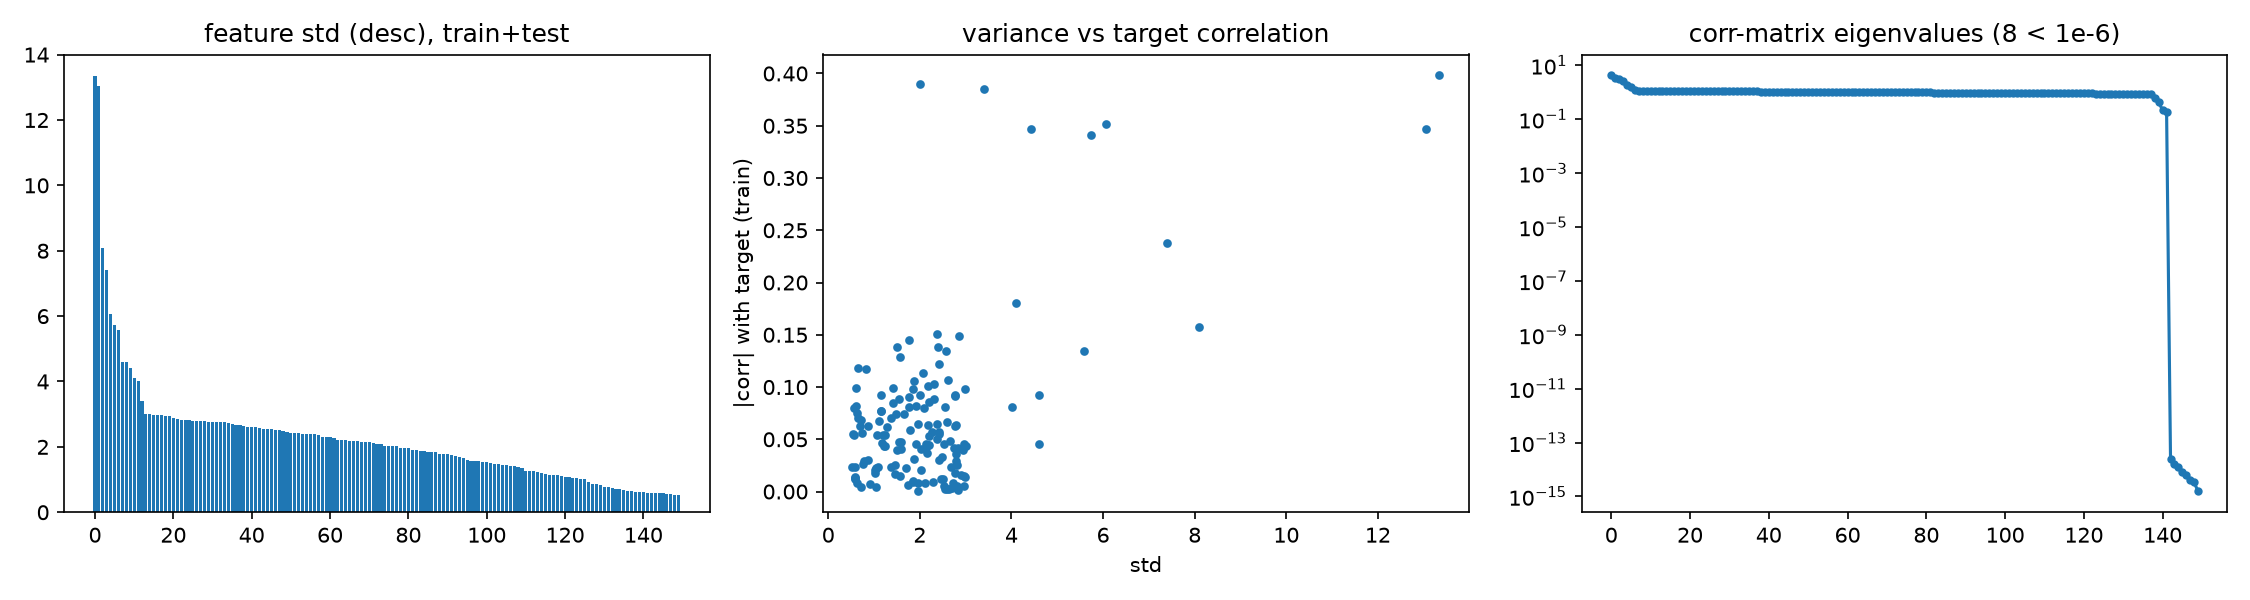
\includegraphics[width=9.0in,trim={0 0 365bp 0},clip]{r001_structure.png}\par
\vspace{0.12in}
\leftbox{9.6in}{%
\begin{itemize}\setlength{\itemsep}{0.06in}
\item \key{13 features}: sd above 1.5 × the median over all 20,000 rows; no labels used.
\item Right: most of the strongest target correlations fall in this block. 130 features are pure noise.
\end{itemize}}
\source{R001 = run 20261022-051627\_r001\_data\_structure (r001\_structure.png, left two panels). R150 = run 20261022-064606\_r150\_taxonomy (130 independent noise columns).}
\end{frame}

%-------------------------------------------------------------------- 4 (protocol)
\begin{frame}{Validation: stratified 5-fold CV, repeated 20 times}
\begin{columns}[T,onlytextwidth]
\column{5.0in}
\vspace{0.02in}
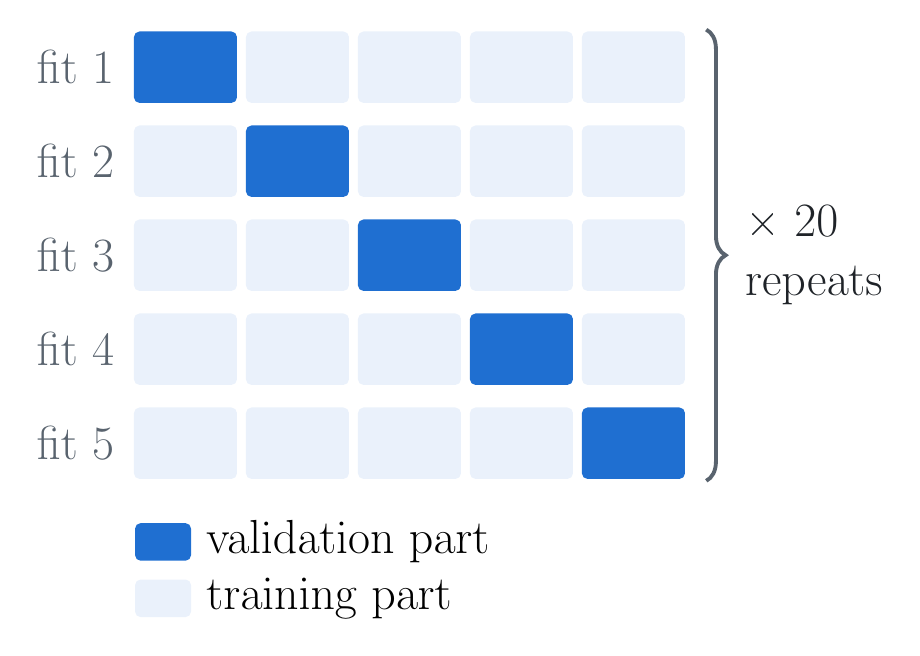
\begin{tikzpicture}[x=0.56in,y=0.47in,font=\fontsize{18}{21}\selectfont]
  \foreach \r in {1,...,5} {
    \node[anchor=east,text=muted] at (0.85,-\r) {fit \r};
    \foreach \c in {1,...,5} {
      \ifnum\r=\c\relax
        \fill[accent,rounded corners=2pt] (\c-0.06,-\r-0.38) rectangle (\c+0.86,-\r+0.38);
      \else
        \fill[soft,rounded corners=2pt] (\c-0.06,-\r-0.38) rectangle (\c+0.86,-\r+0.38);
      \fi
    }
  }
  \draw[decorate,decoration={brace,amplitude=7pt},line width=1.4pt,color=muted]
    (6.05,-0.6) -- (6.05,-5.4) node[midway,right=10pt,align=left,text=ink] {× 20\\repeats};
  \fill[accent,rounded corners=2pt] (0.95,-6.25) rectangle (1.45,-5.85);
  \node[anchor=west] at (1.5,-6.05) {validation part};
  \fill[soft,rounded corners=2pt] (0.95,-6.85) rectangle (1.45,-6.45);
  \node[anchor=west] at (1.5,-6.65) {training part};
\end{tikzpicture}
\column{7.2in}
\begin{itemize}\setlength{\itemsep}{0.20in}
\item New shuffle per repeat (seed 2026 + r): \key{100 validation folds} per model.
\item Scaling, selection and tuning are refitted in each training part. Label-free steps may also use the test features.
\item Models are compared on the same 100 folds. A win needs a gap above 2 split SE \emph{and} corrected p < 0.05.
\item Public leaderboard: a bug check. Every upload was pre-registered.
\end{itemize}
\end{columns}
\source{D002; docs/VALIDATION\_PROTOCOL.md; scripts/compare\_runs.py (Nadeau \& Bengio, 2003). E1 (run 20261022-064054\_e1\_validation\_protocol): 5 × 20 is the only scheme whose minimum detectable difference has a 95\,\% CI below 0.01.}
\end{frame}

%-------------------------------------------------------------------- 5 (E1)
\ifEone
\begin{frame}{E1: only 5-fold × 20, paired, resolves a 0.01 AUC gap}
\framesubtitle{Extension E1 · \OwnerEone}
\begin{columns}[T,onlytextwidth]
\column{7.7in}
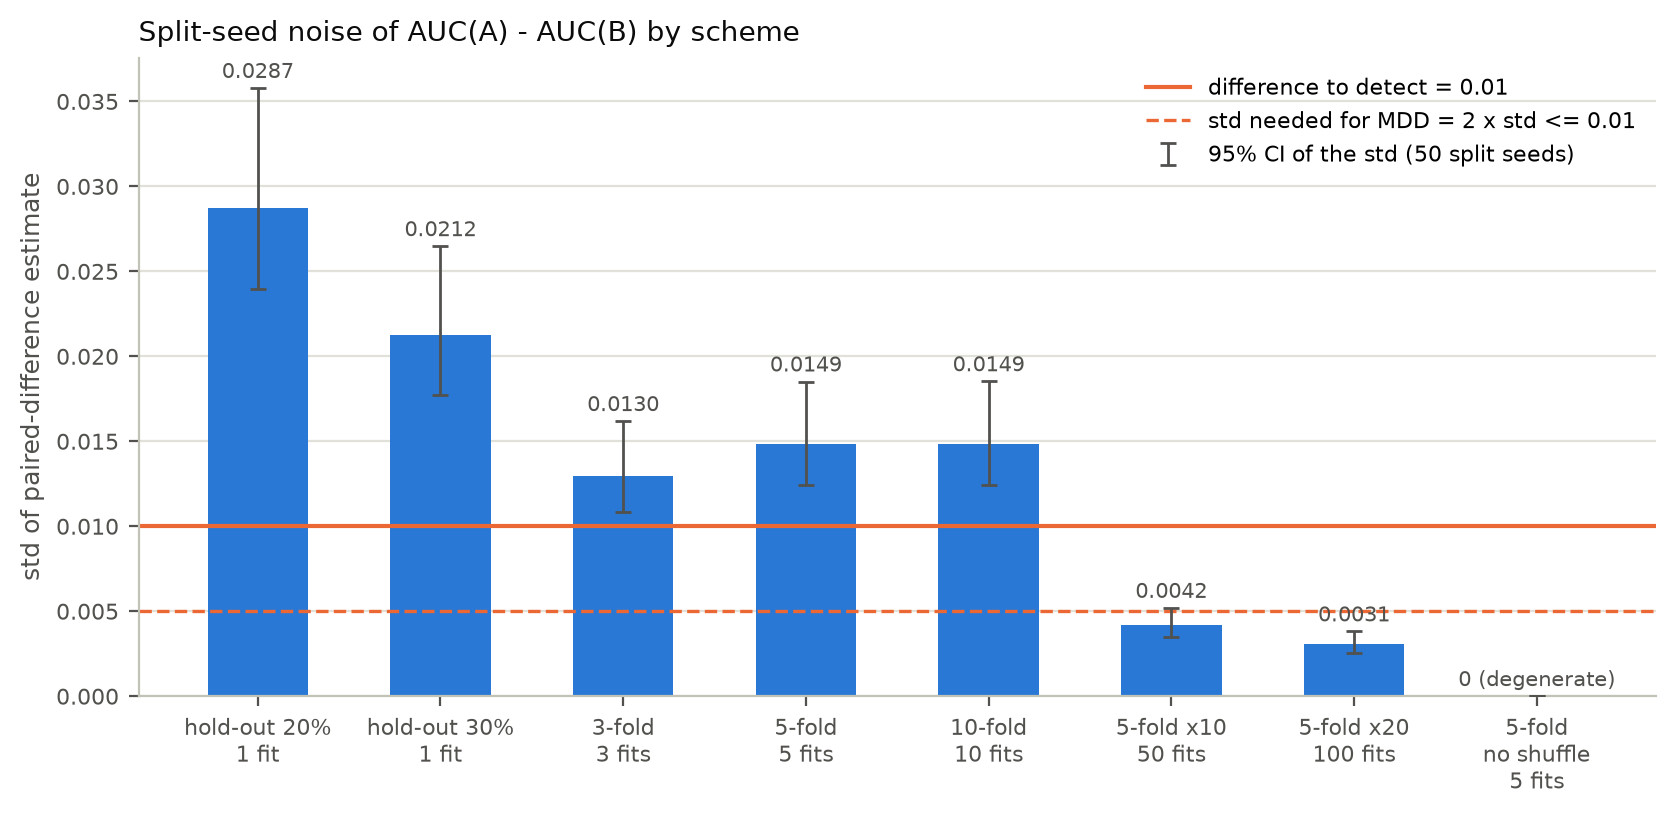
\includegraphics[width=7.65in]{e1_diff_std_by_scheme.png}
\column{4.5in}
\begin{itemize}\setlength{\itemsep}{0.14in}
\item Which scheme can tell apart two models 0.01 AUC apart?
\item 50 split seeds per scheme; model seeds fixed.
\item Minimum detectable difference \mbox{(2 sd)}:\\
  hold-out 20\,\%: 0.057\\ one 5-fold: 0.030\\ 5-fold × 20: \key{0.0061}
\end{itemize}
\end{columns}
\vspace{0.10in}
\leftbox{9.4in}{\callout{\bigtext{Answer: 5-fold × 20, both models on the same splits.}}}
\source{Runs 20261022-064054\_e1\_validation\_protocol, 20261022-064148\_e1\_validation\_protocol\_qda\_pair; e1\_paired\_difference.csv (MDD 0.0061, 95\,\% CI 0.0051--0.0076).}
\end{frame}
\fi

%-------------------------------------------------------------------- 6 (journey)
\begin{frame}{Six uploads, each pre-registered: all within 1.4 SE}
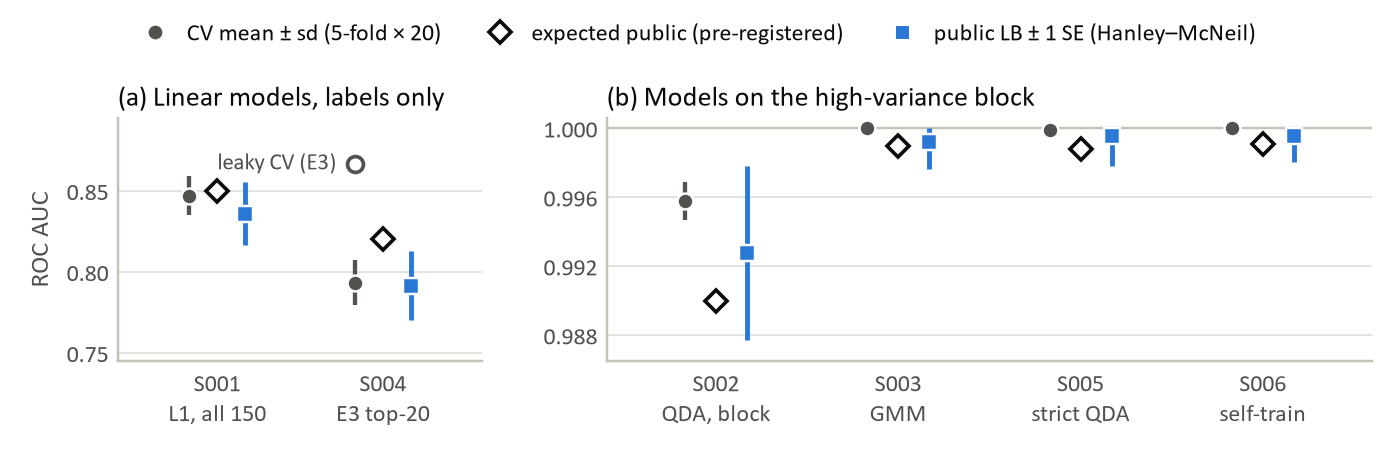
\includegraphics[width=10.6in]{core_journey.png}\par
\vspace{0.06in}
\leftbox{9.4in}{Each expected score (diamond) was written down \emph{before} the upload.}
\source{registry/submissions.csv (S001--S006), registry/beliefs.md (B001--B007); figure and reports/tables/core\_journey.md by scripts/make\_core\_figures.py.}
\end{frame}

%-------------------------------------------------------------------- 7 (journey)
\begin{frame}{What each upload taught us}
\vspace{0.02in}% starts the frame in vertical mode (beamer inserts the title at the first paragraph)
{\renewcommand{\arraystretch}{1.22}
\begin{tabular}{@{}>{\bfseries}l l l l@{}}
\toprule
\mdseries\color{muted}Upload & \color{muted}Model & \color{muted}Public & \color{muted}Lesson\\
\midrule
S001 & L1 logistic, all 150 features & 0.83589 & the CV estimate held\\
S002 & QDA on the 13-feature block & 0.99277 & covariances carry more signal than means\\
S003 & two-cluster mixture (final) & 0.99923 & about 0.999 as predicted; gap: likely label noise\\
S004 & E3 leakage check & 0.79136 & honest CV right; our 0.82 guess too high\\
S005 & strict QDA, labels only & 0.99953 & +0.0003 over S003: noise\\
S006 & self-training QDA & 0.99956 & +0.0003 over S003: noise\\
\bottomrule
\end{tabular}}

\vspace{0.24in}
\leftbox{9.4in}{0.0003 AUC ≈ 12 of the ≈ 39,000 positive–negative pairs in the public set; public gaps have sd 3–6 × 10\textsuperscript{−4}.}
\source{registry/submissions.csv; registry/beliefs.md B001--B007; QDA 0.9958 vs LDA 0.878 in CV: R003 runs 20261022-0506xx\_r003\_*; public-gap sd: R936 (20261022-172146\_r936\_final\_selection).}
\end{frame}

%-------------------------------------------------------------------- 8 (E2)
\ifEtwo
\begin{frame}{E2: more rows help the linear baseline, not the mixture}
\framesubtitle{Extension E2 · \OwnerEtwo}
\begin{columns}[T,onlytextwidth]
\column{7.45in}
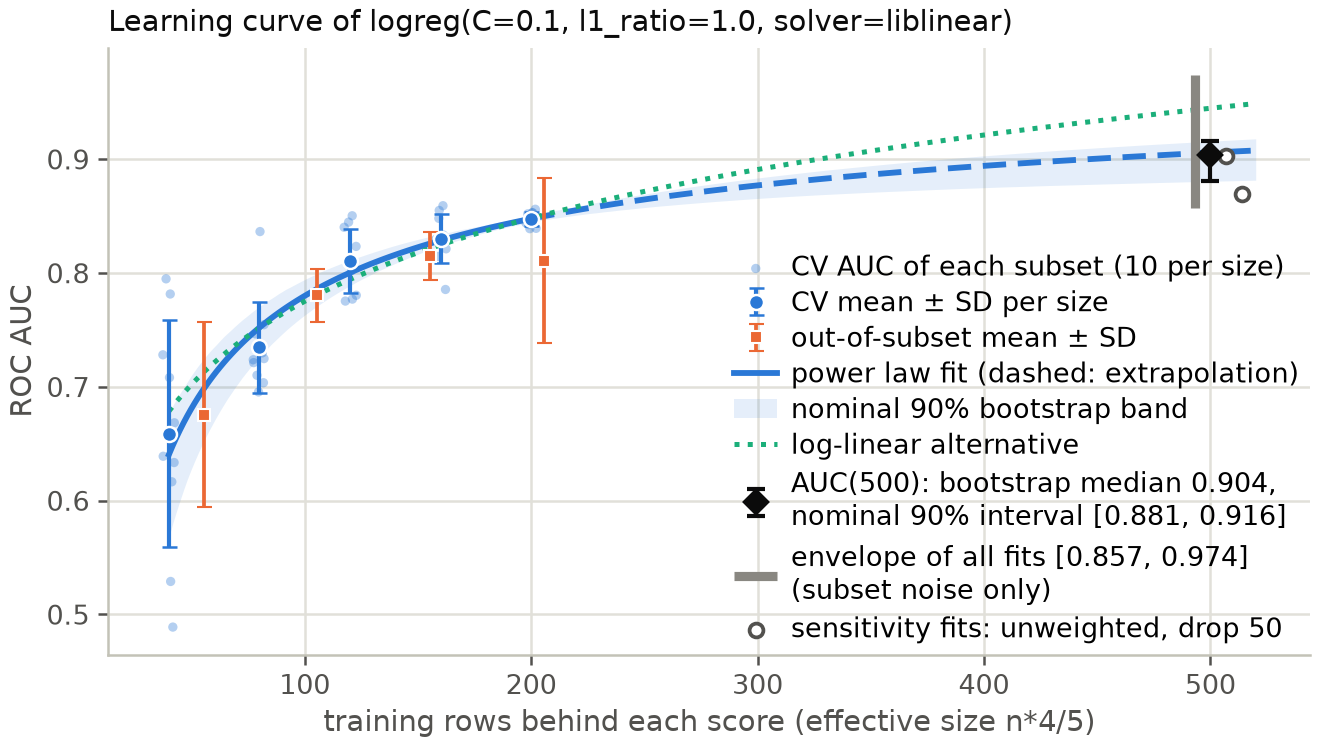
\includegraphics[width=7.4in]{e2_learning_curve.png}
\column{4.75in}
\begin{itemize}\setlength{\itemsep}{0.14in}
\item 10 random subsets per size, 50 to 250 rows.
\item L1 logistic: 0.659 → 0.847. Power law at 500 rows: \key{≈ 0.91}.
\item Its nominal 90\,\% interval held the truth in only 21\,\% of replicas: quote \mbox{\key{± 0.04}}.
\item QDA: 0.973 → 0.996. Mixture: 1.000 at every size.
\end{itemize}
\end{columns}
\source{Runs 20261022-070248\_e2\_learning\_curve, 20261022-070339\_e2\_learning\_curve\_qda\_block, 20261022-070445\_e2\_learning\_curve\_gmm; coverage check R942 (20261022-094142\_r942\_e2\_coverage).}
\end{frame}
\fi

%-------------------------------------------------------------------- 9 (E3)
\ifEthree
\begin{frame}{E3: picking 20 features on all rows inflates CV by 0.07}
\framesubtitle{Extension E3 · \OwnerEthree}
\begin{columns}[T,onlytextwidth]
\column{7.05in}
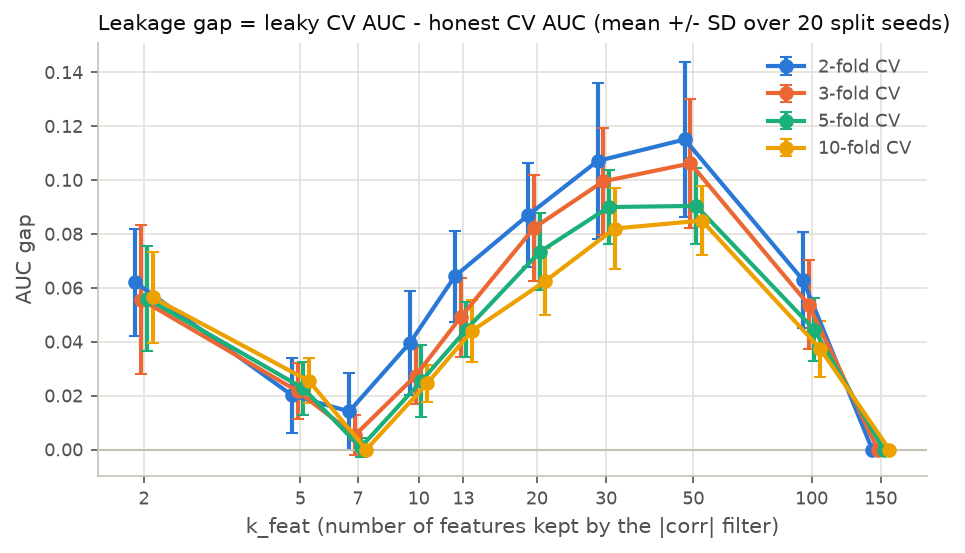
\includegraphics[width=7.0in]{e3_gap_vs_kfeat.png}
\column{5.15in}
{\color{muted}20 features by |corr|, 5-fold CV:}\par\vspace{0.10in}
{\renewcommand{\arraystretch}{1.25}\fontsize{24}{29}\selectfont
\begin{tabular}{@{}l r@{}}
leaky CV (filter on all rows) & \textcolor{accent2}{\bfseries 0.867}\\
honest CV (filter in each fold) & \textcolor{accent}{\bfseries 0.793}\\
public score, S004 & \bfseries 0.791\\
\end{tabular}}\par
\vspace{0.22in}
Gap ≈ 0 at 7 features; about 0.09 at 30--50.
\end{columns}
\vspace{0.12in}
\leftbox{9.4in}{\callout{\bigtext{Every step that uses labels belongs inside the fold.}}}
\source{Run 20261022-063908\_e3\_leakage (reports/tables/e3\_grid.csv, e3\_leaderboard.csv); S004 and its pre-registration B005.}
\end{frame}
\fi

%-------------------------------------------------------------------- 10 (E4)
\ifEfour
\begin{frame}{E4: stably selected is not the same as useful}
\framesubtitle{Extension E4 · \OwnerEfour}
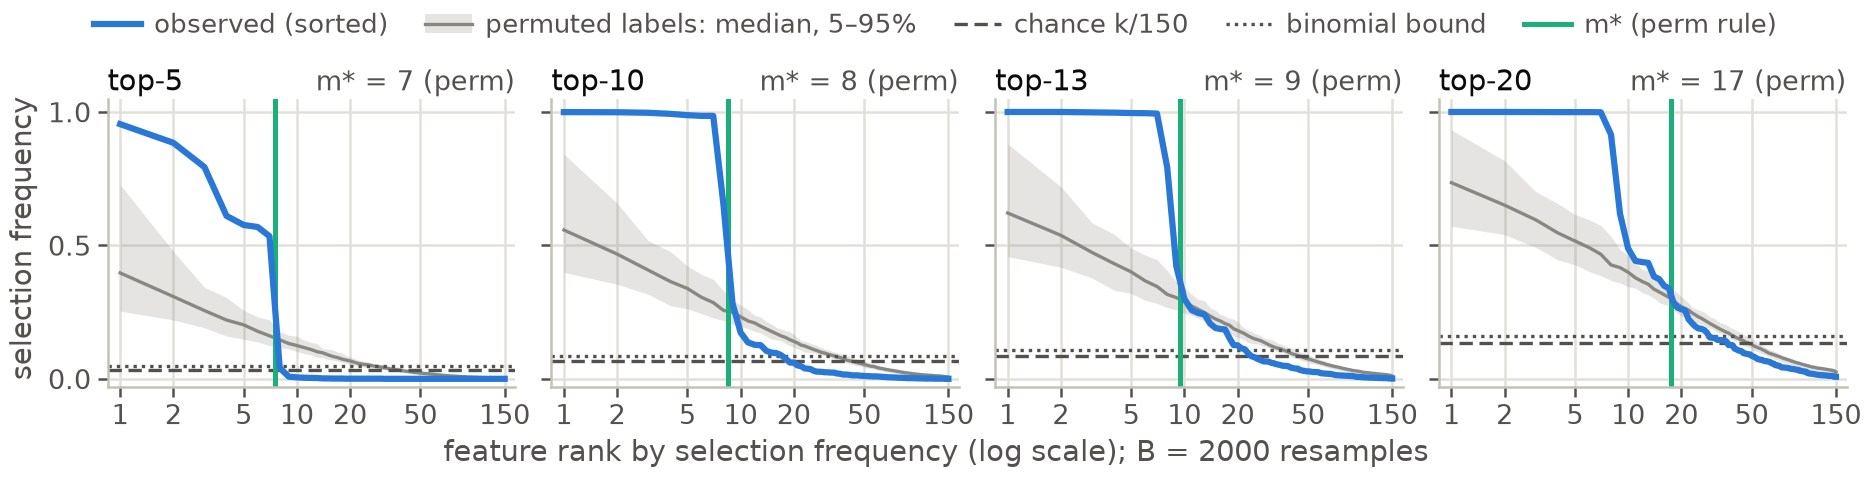
\includegraphics[width=11.2in]{e4_frequency_sorted.png}\par
\vspace{0.12in}
\leftbox{9.6in}{%
\begin{itemize}\setlength{\itemsep}{0.04in}
\item 7 features make the top 10 in ≥ 98.5\,\% of 2,000 resamples; then a sharp drop.
\item Linear model: the stable set adds \key{+0.063} AUC over all 150 features.
\item QDA: stable set \key{0.961}, high-variance block \key{0.996}. Six block features are never stable.
\end{itemize}}
\source{Run 20261022-071414\_e4\_feature\_stability (e4\_frequency.csv, e4\_paired.csv: p = 0.038); R320 = 20261022-074624\_r320\_e4\_stable\_vs\_block (QDA p = 0.0006); R943 null curves.}
\end{frame}
\fi

%-------------------------------------------------------------------- 11 (final solution)
\begin{frame}{Final model (S003): two clusters, fitted without labels}
\begin{columns}[T,onlytextwidth]
\column{7.4in}
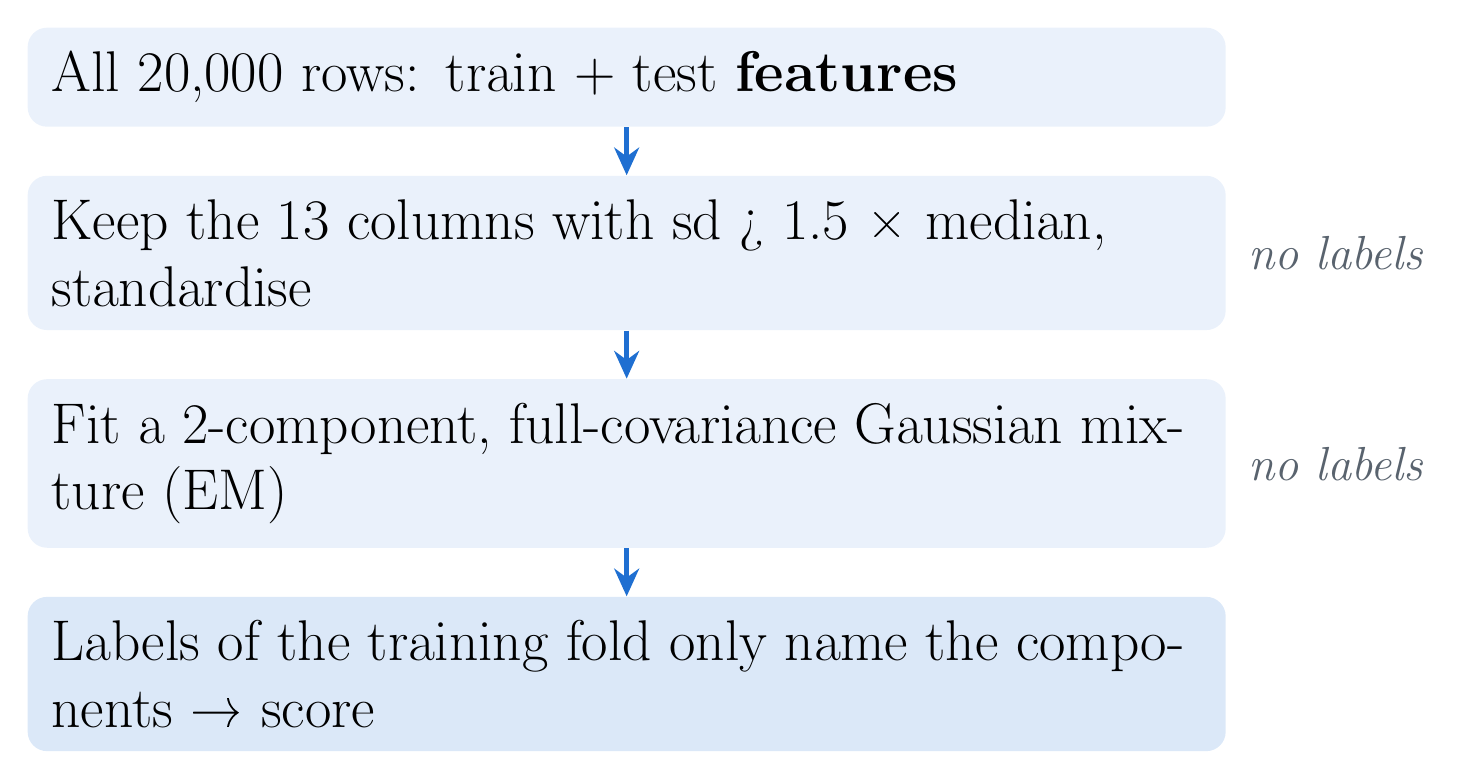
\begin{tikzpicture}[box/.style={fill=soft,rounded corners=7pt,text width=5.75in,inner sep=0.12in,
    align=left,font=\fontsize{20}{24}\selectfont},
  arr/.style={-{Stealth[length=10pt,width=9pt]},line width=2pt,color=accent},
  tag/.style={font=\fontsize{16}{18}\selectfont\itshape,text=muted,anchor=west}]
\node[box] (b1) {All 20,000 rows: train + test \textbf{features}};
\node[box,below=0.24in of b1] (b2) {Keep the 13 columns with sd > 1.5 × median, standardise};
\node[box,below=0.24in of b2] (b3) {Fit a 2-component, full-covariance Gaussian mixture (EM)};
\node[box,below=0.24in of b3,fill=accent!16] (b4) {Labels of the training fold only name the components → score};
\draw[arr] (b1) -- (b2); \draw[arr] (b2) -- (b3); \draw[arr] (b3) -- (b4);
\node[tag] at ([xshift=0.06in]b2.east) {no labels};
\node[tag] at ([xshift=0.06in]b3.east) {no labels};
\end{tikzpicture}
\column{4.8in}
\begin{itemize}\setlength{\itemsep}{0.16in}
\item CV AUC \key{1.0000} in 100 of 100 folds
\item Public \key{0.99923}
\item No setting tuned on labels
\item Test features are competition data (rule 4, Foundational 18a); no test label is used.
\end{itemize}
\end{columns}
\source{Run 20261022-050708\_r003\_gmm2\_hv; configs/final\_s003\_gmm2\_hv.yaml; bit-identical re-run R910. Rule reading: D007, D014 (the instructor has not confirmed it yet).}
\end{frame}

%-------------------------------------------------------------------- 12 (final solution)
\begin{frame}{Why S003: the unlabelled rows do the work}
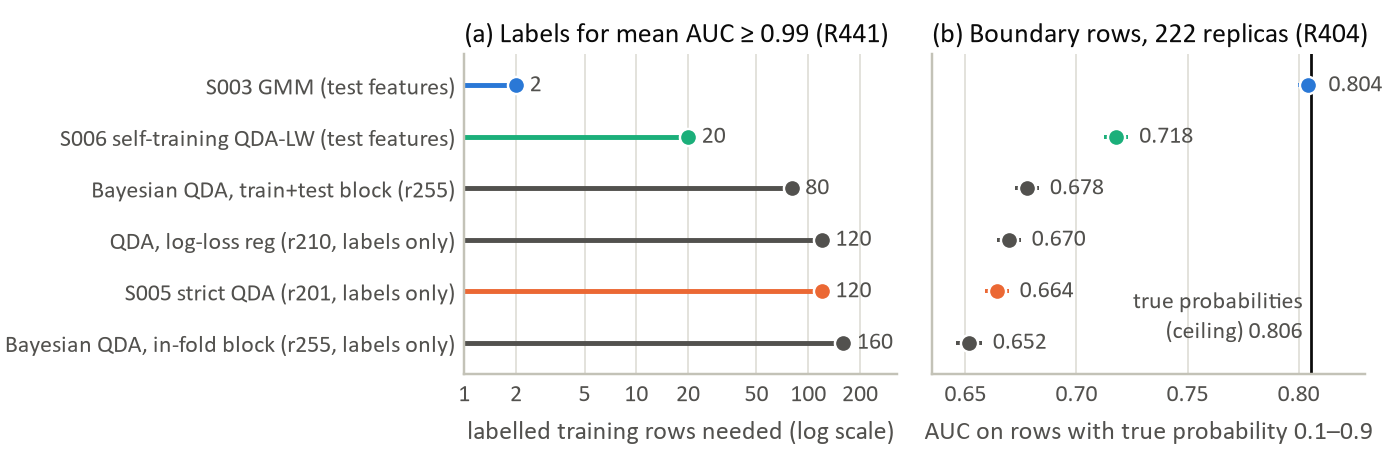
\includegraphics[width=11.3in]{core_unlabeled_value.png}\par
\vspace{0.12in}
\leftbox{9.6in}{%
\begin{itemize}\setlength{\itemsep}{0.04in}
\item BIC, which uses no labels, picks exactly 2 components (R101).
\item On 222 simulated data sets, all others score lower on average (R936).
\end{itemize}}
\source{(a) R441 = 20261022-182022\_r441\_label\_budget\_rerun; (b) R404 = 20261022-194238\_r404\_inductive\_pooled; R101 = 20261022-064201\_r101\_bic\_model\_choice; R936 = 20261022-172146\_r936\_final\_selection.}
\end{frame}

%-------------------------------------------------------------------- 13 (final solution)
\begin{frame}{Final picks: a rule written before the last two scores}
\vspace{0.02in}% see the note on the 'What each upload taught us' slide
{\renewcommand{\arraystretch}{1.3}\fontsize{22}{27}\selectfont
\begin{tabular}{@{}l l@{}}
\toprule
\color{muted}Instructor's answer on test features & \color{muted}Our two final picks\\
\midrule
none yet (default) & \key{S003 + S005}\\
explicitly allowed & S003 + S006\\
forbidden & extended-grid QDA (r930) + S005\\
\bottomrule
\end{tabular}}

\vspace{0.28in}
\begin{itemize}\setlength{\itemsep}{0.14in}
\item Written before the S005 and S006 scores were seen. Public gaps (sd 3–6 × 10\textsuperscript{−4}) cannot change it.
\item S005 never sees the test features: a safe second pick under any reading of the rules.
\item Expected private AUC of S003: about \key{0.997} (90\,\%: 0.992–0.9996), limited by label noise.
\end{itemize}
\source{registry/decisions.md D010 and D013; R936 (20261022-172146\_r936\_final\_selection); R922 (20261022-092146\_r922\_label\_noise\_private).}
\end{frame}

%-------------------------------------------------------------------- 14 (closing, all members)
\begin{frame}{What we take away}
\vspace{0.06in}
{\fontsize{26}{32}\selectfont
\begin{itemize}\setlength{\itemsep}{0.30in}
\ifdefempty{\TakeA}{}{\item \TakeA\\{\fontsize{20}{24}\selectfont\color{muted}\NameA}}
\ifdefempty{\TakeB}{}{\item \TakeB\\{\fontsize{20}{24}\selectfont\color{muted}\NameB}}
\ifdefempty{\TakeC}{}{\item \TakeC\\{\fontsize{20}{24}\selectfont\color{muted}\NameC}}
\end{itemize}}
\vfill
{\fontsize{34}{40}\selectfont\bfseries Thank you\par}
\vspace{0.10in}
\leftbox{9.4in}{\fontsize{15}{18}\selectfont\color{muted}AI use: Claude Code (Anthropic) wrote most of our code, ran the experiments and drafted our texts; see the report.}\par
\vspace*{0.05in}
\end{frame}

\end{document}
